\documentclass[a4paper, 12pt]{article}
\usepackage[utf8]{inputenc}
\usepackage[T1]{fontenc}
\usepackage[margin=2cm]{geometry} % Marges standard de 2cm
\usepackage{fontawesome5}
\usepackage{raleway}
\renewcommand{\familydefault}{\sfdefault}
\usepackage{xcolor}
\usepackage{tikz}

% --- Palette de couleurs Vives ---
\definecolor{colManager}{HTML}{2C3E50}
\definecolor{colTeam}{HTML}{E67E22}
\definecolor{colExt}{HTML}{16A085}
\definecolor{colProcess}{HTML}{8E44AD}
\definecolor{colBack}{HTML}{FDFEFE}

\usetikzlibrary{shapes.geometric, positioning, shadows.blur, calc, arrows.meta}

\begin{document}
\thispagestyle{empty} % Enlève le numéro de page

\begin{center} % Centre l'organigramme sur la page A4
    \begin{tikzpicture}[
        node distance=1cm,
        spine/.style={line width=3pt, draw=black!10, cap=round},
        hexNode/.style={
            regular polygon,
            regular polygon sides=6,
            minimum size=4.5cm,
            inner sep=0pt,
            fill=colManager,
            text=white,
            align=center,
            blur shadow={shadow blur steps=5},
            font=\bfseries
        },
  % Nœud Equipe (Droite)
    rightNode/.style={
        rectangle,
        rounded corners=15pt,
        fill=colTeam,
        text=white,
        align=left,
        text width=6cm,
        inner sep=12pt,
        anchor=west,
        blur shadow,
        font=\small
    },
        leftNode/.style={
            rectangle,
            rounded corners=15pt,
            fill=colExt,
            text=white,
            align=right,
            text width=5.5cm,
            inner sep=12pt,
            anchor=east,
            blur shadow,
            font=\small
        },
        bottomNode/.style={
            rectangle,
            rounded corners=8pt,
            draw=colProcess,
            line width=2pt,
            fill=white,
            text=colProcess,
            align=left,
            text width=12cm,
            inner sep=10pt,
            font=\small
        },
        connect/.style={
            draw=black!30,
            line width=1.5pt,
            -{Circle[width=3pt,length=3pt]}
        }
    ]

        % --- 0. DÉCORATION D'ARRIÈRE-PLAN ---
        \fill[colManager!5] (0,0) circle (3.5cm);

        % --- 1. L'Axe Central ---
        \draw[spine] (0, 3.5) -- (0, -11.5);

        % --- 2. Header (Contact) ---
        \node[fill=white, text=black!70, draw=black!10, rounded corners=5pt, inner sep=8pt, align=center] (contact) at (0, 4) {
            \faIcon{address-card} \textbf{CONTACT UNIQUE}\\
            03.89.53.36.58 $\mid$ 06 24 18 26 89\\
            \textit{contact@bois-techniques.fr}
        };

        % --- 3. Le Cœur : Conducteur ---
        \node[hexNode] (manager) at (0,-2.5) {
            \faIcon{user-tie} \\[0.2cm]
            \large Frederic ANSELM\\
            \footnotesize DIRECTEUR D'EXPLOITATION\\[0.1cm]
            \small 17 ans d'expérience\\
            \small BTS Const. Bois Habitat
        };

    % --- 4. Branche Droite : L'Action (Équipe) ---
    \node[rightNode] (team) at (2.2, -6.2) {
        \textbf{\faIcon{tools} ÉQUIPE TRAVAUX N°1}\\[0.2cm]
        \textbf{Jimmy FROGER} (Chef)\\
        \small 22 ans exp. - CAP Charpentier/Menuisier\\[0.15cm]
        \normalsize \textit{Renforts : \\ Thomas NEFF}
    };


        % --- 5. Branche Gauche : Externe ---
        \node[leftNode] (ext) at (-3, -4.2) {
            \textbf{RELATIONS EXTÉRIEURES \faIcon{project-diagram}}\\[0.2cm]
            Maîtrise d'Ouvrage\\
            Architecte (maîtrise d'œuvre, OPC)\\
            Bureaux d'Études\\
            Organismes (SPS, Inspection\\du travail, bureau de contrôle...)\\
            Entreprises en charge\\des autres lots
        };

        % --- 6. Branche Gauche Basse : Prestataires ---
        \node[leftNode, fill=colExt!80!black, text width=4.5cm] (prest) at (-2.5, -10.5) {
            \textbf{PRESTATAIRES CLÉS \faIcon{truck}}\\[0.1cm]
            \textbf{SCHROLL :} Déchets\\
            \textbf{MEDIACO :} Levage Lourd
        };

        % --- 7. Le Processus (MODIFIÉ) ---
        \node[bottomNode] (process) at (0, -15.5) {
            \centering \textbf{\faIcon{sync-alt} SUIVI DE CHANTIER \& EFFECTIFS}\\[0.2cm]
            
            \raggedright
            \textbf{\small 1. Réunion quotidienne (7h30 A.M) :}\\\textit{Avant le départ sur les chantiers}\\
            \begin{itemize}
                \setlength\itemsep{0em}
                \item Échangés sur l'avancement, problèmes rencontrés ou risques (info autres lots, MOE...).
                \item Explication sur la suite des travaux (mise en garde sécuritaire si besoin).
                \item Adaptation suite à des modifications en cours de chantier.
            \end{itemize}
            
            \vspace{0.1cm}
            \vspace{0.1cm}

            \textbf{\small 2. Gestion des effectifs :}\\
            \textbf{Effectif estimé :} 2 à 4 personnes.\\
            \textbf{Augmentation de l’effectif :} Possibilité d’accroître les effectifs en fonction du planning ou des difficultés.
        };

        % --- 8. LIENS ---
        \draw[connect, color=colTeam] (manager.east) to[out=0,in=130] (team.north west);
        \draw[connect, color=colExt] (manager.west) to[out=180,in=50] (ext.north east);
        \draw[connect, color=colExt!80!black] (0,-7) -- (prest.east);
        \node[fill=white, inner sep=2pt] at (0,-9) {\textcolor{colProcess}{\faIcon{arrow-down}}};

    \end{tikzpicture}
\end{center}
\end{document}